\hthree{REST-Prinzipien}

Grundsätzlich muss eine REST-API sechs bestimmte Eigenschaften aufweisen, um als REST-API zu gelten. Dabei ist jedoch nicht festgelegt, wie diese Eigenschaften implementiert werden. \cite{RedHatRest}

\hfour{Client-Server Prinzip}

Das Client-Server Prinzip ist eine spezielle Art und Weise, wie zwei Systeme miteinander kommunizieren. Bei diesem Prinzip haben die Kommunikationspartner zwei unterschiedliche Aufgaben, beziehungsweise Rollen. Das Client-Server-Prinzip basiert auf dem Gedanken, dass einer der beiden Systeme (Client) Informationen von seinem Kommunikationspartner anfordert. Der Server antwortet daraufhin. Die Anfrage, die der Client schickt, wird auch Request genannt, die Antwort des Servers wird Response genannt. Heutzutage wird das Client-Server-Prinzip am häufigsten angewendet, jedoch gibt es bis heute Fälle, in denen zum Beispiel Peer-To-Peer-Kommunikationen bevorzugt werden.

Grundsätzlich gibt es drei verschiedene Arten, wie ein Client mit einem Server innerhalb des Client-Server-Prinzips kommuniziert. 

\begin{figure}[H]
    \centering
    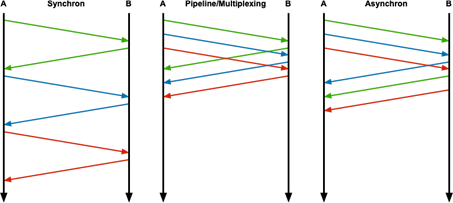
\includegraphics[width=0.9\textwidth]{media/REST/ClientServer.png}
    \caption{Verschiedene Kommunikationsschemata \cite{ClientServer}}
\end{figure}

Bei der synchronen Kommunikation schickt der Client dem Server einen Request. Der Server antwortet entsprechend auf diesen Request, nachdem er den Request erhält. Nachdem der Client die Response vom Server bekommen hat, kann er nun wieder einen Request schicken. Die Kommunikation läuft also synchron ab.

Beim sogenannten Multiplexing schickt der Client hintereinander mehrere Requests an den Server, ohne nach jedem Request auf die Antwort des Servers zu warten. Nachdem der Client alle Requests an den Server geschickt hat, wartet er auf alle Antworten. Wenn der Server die erste Anfrage bekommt, bearbeitet er diese Anfrage und schickt eine Antwort zurück an den Client. Erst wenn die erste Anfrage vollständig bearbeitet wurde, kümmert sich der Server um die nächste Anfrage.

Bei der sogenannten asynchronen Kommunikation schickt der Server wie beim Multiplexing mehrere Requests hintereinander an den Server. Der Server bearbeitet diese Anfragen dann asynchron statt synchron. Dies bedeutet, dass die Bearbeitung einer Anfrage die Bearbeitung einer anderen Anfragen nicht blockiert. Die verschiedenen Anfragen werden praktisch unabhängig voneinander bearbeitet. Durch diese asynchrone Arbeitsweise ist es zum Beispiel möglich, dass der Request, der als letztes zum Server geschickt wird, als erstes beantwortet wird, da seine Bearbeitung die geringste Zeit beansprucht. \cite{ClientServer}

\hfour{Zustandslosigkeit}

Zustandslosigkeit im REST-Kontext bedeutet, dass jede Anfrage beziehungsweise Antwort alle Informationen benötigt, um diese zu verstehen. Eine REST-Anfrage besteht somit nur aus einer einzigen Anfrage und nicht aus mehreren, voneinander abhängigen Anfragen. Dieses Prinzip gilt auch für alle Antworten des Servers. Vorteile dieser Zustandslosigkeit ist die einfache Skalierbarkeit eines Servers. Dies begünstigt beispielsweise die Lastverteilung von Anfragen auf mehrere Server. Da es während der Client-Server Kommunikation nicht mehrere Zustände gibt, entfällt die Notwendigkeit einer serverseitigen Verwaltung von Sitzungen. Bestimmte Anwendungsinformationen werden nur noch clientseitig mithilfe von Cookies und anderen Techniken gespeichert. Ein weiterer wichtiger Vorteil der Zustandslosigkeit ist die Steigerung der Ausfallssicherheit, da die Datenübertragung mit einem einzigen Request und einer einzigen Response erfolgt. Der gravierende Nachteil dieses Prinzips ist die Verschlechterung der Netzwerkperformance, da durch die Zustandslosigkeit alle notwendigen Informationen mit einem einzigen Request beziehungsweise Response geschickt werden. Dadurch ist die Komplexität und Größe von REST-Nachrichten größer als bei zustandsabhängigen Protokollen. \cite{WikiREST}

\hfour{Caching}

REST-Anwendungen sollen, wenn möglich, HTTP-Caching verwenden. Jedoch gilt: so wenig Anfragen wie möglich. Der Nachteil dabei ist aber, dass möglicherweise veraltete Daten aus dem Cache aufgegriffen werden, wenn zu sparsam mit Anfragen umgegangen wird. \cite{WikiREST}

\hfour{Einheitliche Schnittstelle}

Eines der wichtigsten Merkmale einer REST-Applikation ist eine einheitliche Schnittstelle. Diese sichert die einfache Nutzung von REST-Applikationen. Die Vereinheitlichung besteht aus den vier folgenden Eigenschaften:

\pagebreak

\hfive{Ressourcen und deren Adressierung}

Alle Informationen, die über eine URL erreichbar sind, werden Ressourcen bezeichnet. Generell kann jede REST-Anwendung über eine eindeutige URL erreicht werden. \cite{WikiREST}

\hfive{Darstellung von Ressourcen}

Auf einem REST-konformen Server können unterschiedliche Dienste unterschiedliche Darstellungsformen (Repräsentationen) einer Ressource haben. Beispielsweise kann ein Server eine Ressource in HTML, JSON oder XML anbieten. Die Veränderung einer Ressource erfolgt stets nur über eine Repräsentation. \cite{WikiREST}

\hfive{Selbstbeschreibende Nachrichten}

Alle Requests und Responses in einer REST-Anwendung müssen selbstbeschreibend sein. Damit man dies erreicht, verwenden REST-Anwendungen Standardmethoden, um Ressourcen zu manipulieren. Die am meisten verbreiteten Methoden sind die HTTP-Methoden. Folgende HTTP-Methoden werden bei REST verwendet:

\begin{itemize}
    \item GET -- Mit GET wird eine Ressource vom Server angefordert. Dabei wird am serverseitigen Zustand nichts verändert, wodurch GET als sichere HTTP-Methode gilt.
    \item POST -- Mit POST wird eine Subressource unterhalb der angegebenen Ressource auf dem Server erstellt werden. Ein neuer Ressourcenlink wird erstellt und an den Client zurückgeliefert.
    \item PUT -- Mit PUT wird die angegebene Ressource erstellt. Wenn die angegebene Ressource bereits existiert, wird sie abgeändert. 
    \item PATCH -- Mit PATCH wird ein Teil der angegebenen Ressource geändert. 
    \item DELETE -- Mit DELETE wird die angegebene Ressource gelöscht.
    \item HEAD -- Mit HEAD werden Metadaten zu der angegebenen Ressource angefordert. 
    \item OPTIONS -- Mit OPTIONS werden die erlaubten HTTP-Methoden für die angegebene Ressource abgefragt. 
    \item CONNECT -- Mit CONNECT wird die Anfrage durch einen TCP-Tunnel geleitet. 
    \item TRACE -- Mit TRACE kann überprüft werden, ob sich an der Anfrage am Weg zum Server etwas ändert. Dabei schickt der Server die Anfrage, wie er sie bekommen hat zum Client zurück. Nun kann diese Anfrage mit der Anfrage, die der Client weggeschickt hat, verglichen werden. 
\end{itemize}

Optional können weitere HTTP-Befehle wie COPY, MOVE, MKCOL, LOCK, UNLOCK, LINK und UNLINK verwendet werden. Falls UDP mit REST verwendet wird, kann das Constrained Application Protocol verwendet werden, welches leicht abgeänderte GET-, POST-, PUT- und DELETE-Methoden besitzt. \cite{WikiREST}
